\documentclass{article}

\usepackage[preprint,nonatbib]{../neurips_2024}
\usepackage[utf8]{inputenc}
\usepackage[T1]{fontenc}
\usepackage{hyperref}
\usepackage{url}
\usepackage{booktabs}
\usepackage{graphicx}
\usepackage{amsmath}
\usepackage{amsfonts}
\usepackage{xcolor}
\usepackage{enumitem}
\usepackage{multirow}
\usepackage{tabularx}
\usepackage{array}
\usepackage{placeins}
\hypersetup{hidelinks}

\graphicspath{{presentation/figures/}{../}}

\makeatletter
\renewcommand{\@notice}{}
\makeatother

\newcommand{\method}[1]{\texttt{\detokenize{#1}}}
\newcommand{\dataset}[1]{\textsc{#1}}

\title{Bottleneck-Typed Retrieval for Legal and Multi-Hop Question Answering}

\author{%
  Hamza Iqbal \\
  Washington University in St.\ Louis \\
  \texttt{hiqbal@wustl.edu}
  \And
  Hanson Li \\
  Washington University in St.\ Louis \\
  \texttt{hanson.l@wustl.edu}
  \And
  Josh Li \\
  Washington University in St.\ Louis \\
  \texttt{josh.l@wustl.edu}
}

\begin{document}

\maketitle

\begin{abstract}
RAG should be selected as a bottleneck-targeted intervention: top-$k$
sensitivity diagnoses whether the active failure is retrieval depth, query
formulation, evidence use, or answer-option anchoring. We began with a full
LangGraph legal RAG agent, but exploratory results showed that extra planning
and retrieval could distract models with strong legal priors. We therefore
reframed the project around a bottleneck-typed evaluation across BarExam,
MuSiQue, CaseHOLD, LegalBench-SCALR, and HousingQA. The same retrieval-depth
policy stress test separates regimes. On Llama 70B MuSiQue, restricting
\method{rag_simple} from top-5 to top-1 passages drops EM from 27.5\% to
13.0\% (-14.5pp, McNemar $p=4.18\times10^{-7}$). On an N=200 Gemma 4 26B
BarExam diagnostic, the analogous top-5/top-1 comparison is flat (82.5\% to
83.0\%, $p=1.00$). LegalBench-SCALR is candidate-depth sensitive (77.0\% to
59.5\% at top-1), while HousingQA is a promising but directional statutory
replicate (50.5\% top-1 to 58.0\% top-10, $p=0.0722$). Snap-HyDE is used as a
probe, not the novelty claim: on MuSiQue it improves Llama 70B from 27.5\% to
37.0\% (+9.5pp, $p=0.0079$), while BarExam's full-corpus Gemma 4 26B
\method{rag_snap_hyde} result improves from 78.08\% to 81.17\% ($N=1195$).
The central lesson is not that one RAG method wins, but that retrieval methods
should be chosen according to the benchmark-model bottleneck.
\end{abstract}

\section{Introduction}

Legal question answering is a difficult testbed for RAG. The model must apply
rules, exceptions, and fact patterns precisely, and the retrieved text may be
only partially aligned with the issue in the question. Our original project
therefore built an agentic legal RAG system: a classifier/planner decomposed a
question, an executor retrieved and synthesized evidence for each step, an
evaluator judged whether evidence was sufficient, and a replanner added or
revised steps when the evidence was incomplete.

The first lesson was negative but useful. In exploratory BarExam checks, the
full agentic loop was expensive and did not reliably outperform direct model
answering. We treat those early rows as motivation rather than signed-off
evidence. They exposed the broader problem that more retrieval and more agent
structure can distract a model that already has strong priors, while also
fragmenting reasoning across multiple calls.

We pivoted from ``build the largest agent'' to ``measure which bottleneck is
active.'' The result is a bottleneck-typed account of RAG. Some benchmark-model
pairs are \emph{retrieval-depth limited}: answer accuracy is sensitive to
whether enough useful passages are retrieved. Others are \emph{depth-flat}:
the useful intervention is answer anchoring or option calibration, not more
documents. Holding-selection tasks split further: SCALR is candidate-depth
limited until top-5, while CaseHOLD is answer-flat under the current harness
and still needs repaired retrieval-recall instrumentation.

This framing also explains why a seemingly weak control, \method{golden_passage},
can underperform \method{llm_only} and \method{rag_snap_hyde} on BarExam.
Providing a single labeled passage is not an oracle ceiling. In our full
Gemma 4 26B BarExam audit, \method{golden_passage} flips 96 previously correct
\method{llm_only} answers to wrong and only 83 wrong answers to correct. The
gold passage often anchors the model on a related but incomplete rule. In
contrast, the pattern is consistent with snap-first methods preserving useful
legal priors before evidence reconciliation, which is why
\method{snap_only_in_final} and \method{rag_snap_hyde} both beat the forced
gold-passage control.

\section{Related Work}

Our method is related to generated-query and draft-conditioned retrieval.
HyDE generates a hypothetical document and embeds it for zero-shot dense
retrieval \cite{hyde2023}. Query2Doc similarly uses LLM-generated pseudo
documents for query expansion \cite{query2doc2023}. FLARE retrieves using
tentative generated text during long-form generation \cite{flare2023}, while
Iter-RetGen and CoRAG iterate between generation and retrieval
\cite{iterretgen2023,corag2025}. Speculative RAG uses multiple retrieved
document subsets to draft answers and a verifier to select among them
\cite{specrag2025}. Our snap-HyDE variant is simpler and fixed-cost: one call
produces a tentative answer and a retrieval passage, and a second call
synthesizes the final response.

The more important distinction is the bottleneck framing. Adaptive-RAG routes
questions by complexity \cite{adaptiverag2024}; Know Your RAG and GRADE
classify question difficulty and multi-hop structure \cite{knowyourrag2025,
grade2025}. Legal RAG benchmarks have already shown that retrieval helps some
legal tasks and hurts others. Zheng et al.\ introduce BarExam QA and HousingQA
and report that retrieval helps Housing much more than BarExam
\cite{zheng2025legalretrievalbench}. Vaddi reports task-dependent legal RAG
behavior, including gains on ContractNLI and degradation on CaseHOLD
\cite{vaddi2026legal}. We build on these observations by treating retrieval
benefit as a measurable bottleneck signature rather than a universal property
of the retriever.

This boundary matters. We do not claim that snap-HyDE is fundamentally novel
relative to HyDE, generated-query retrieval, or active retrieval. Instead, the
contribution is a diagnostic matrix: no-context, top-1/top-5 retrieval,
single gold-passage controls, generated-query methods, and snap-anchored
variants together identify whether a benchmark is retrieval-depth limited,
query-formulation limited, evidence-utilization limited, or answer-option
disambiguation limited.

\section{System and Method}

\subsection{Initial agentic legal RAG system}

The initial system was a LangGraph plan-execute-evaluate loop. A planner
constructed a legal research plan, an executor ran multi-query retrieval and
source-grounded synthesis for each step, a judge checked whether the retrieved
evidence was sufficient, and a replanner added follow-up research steps when
needed. This design was useful for exploring legal-agent architecture, but
the evaluation showed that its many moving pieces made it hard to identify
where accuracy gains or losses came from.

\begin{figure}[!htbp]
  \centering
  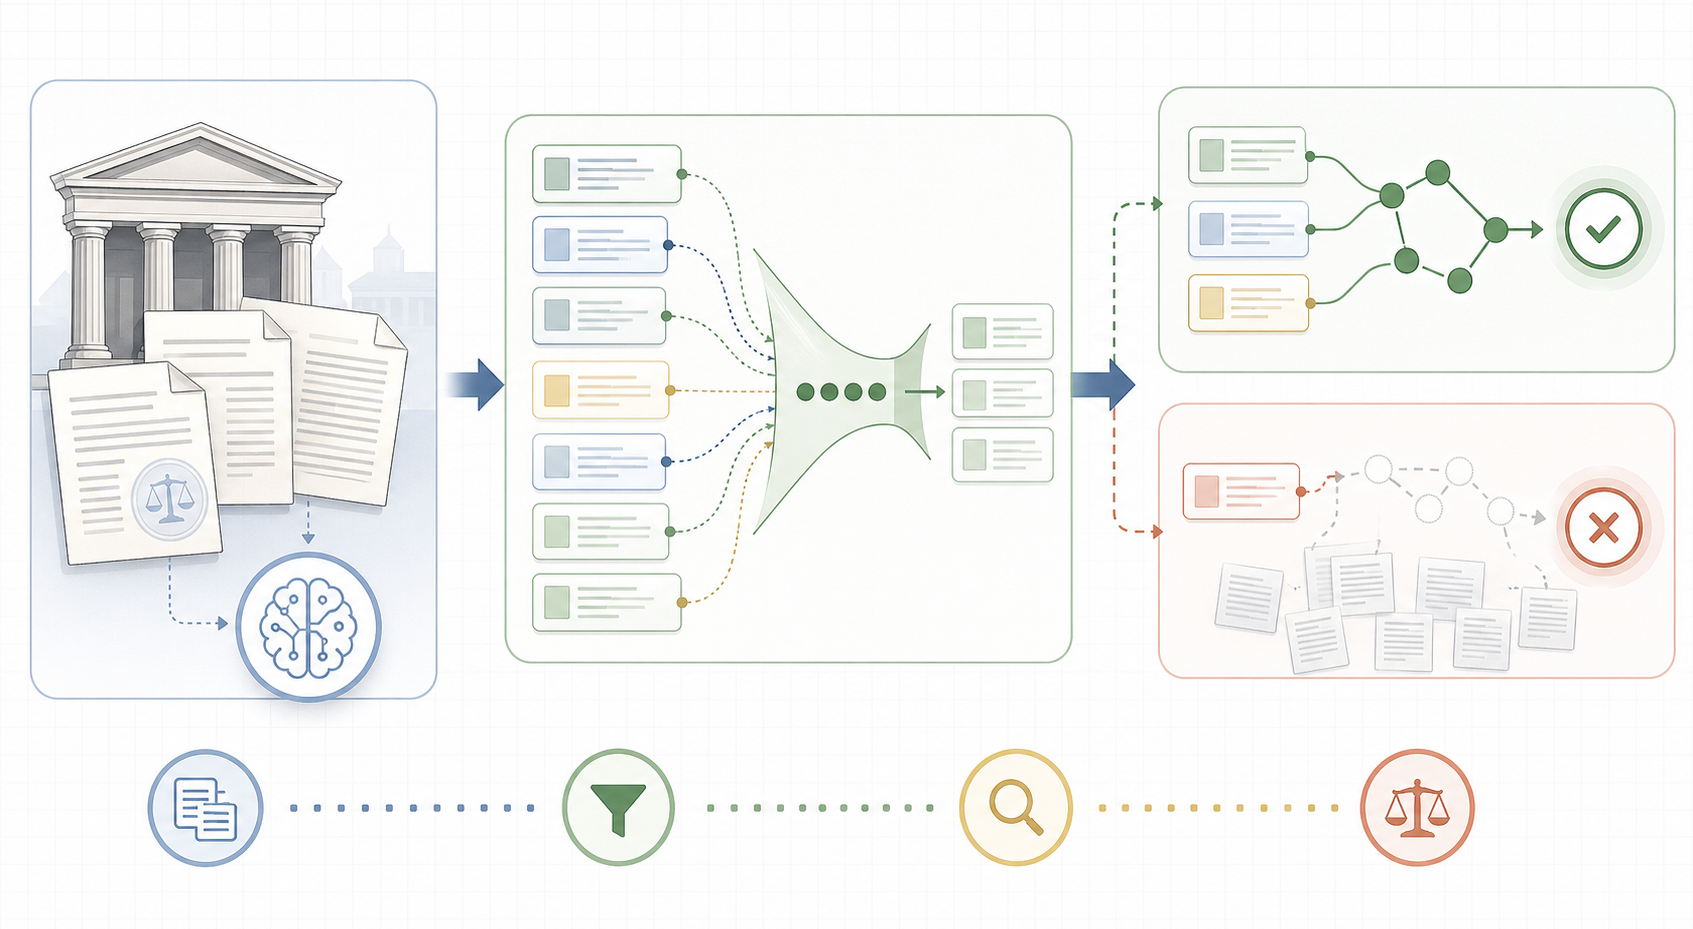
\includegraphics[width=0.94\textwidth]{09_bottleneck_rag_graphical_abstract.png}
  \caption{Project pivot. The initial architecture emphasized a full legal
  research agent. The final experiments sort questions through controlled
  retrieval interventions and ask which bottleneck produces success or failure.}
  \label{fig:pivot}
\end{figure}

\subsection{Snap-conditioned retrieval}

The core method family is snap-conditioned retrieval. In the legal multiple
choice setting, the model first produces a tentative answer or legal analysis.
That snap is then used to guide a HyDE-style passage or evidence query. The
retriever searches with this answer-shaped query, and a final synthesis call
combines the original question, snap, and retrieved passages.

The two-call version, \method{snap_hyde_2call}, makes this fixed-cost:

\begin{enumerate}[leftmargin=*,nosep]
  \item Call 1: produce a tentative answer plus a reference passage stating
  the controlling rule, doctrine, fact, or principle.
  \item Retrieval: embed the generated passage and retrieve the top-$k$
  passages from the corpus.
  \item Call 2: synthesize the final answer using the question, snap, and
  retrieved evidence.
\end{enumerate}

This design is not claimed as a universal invention independent of prior
work. Its value in this project is as a compact probe: when it helps, we can
ask whether the gain came from better retrieval recall, stronger answer
anchoring, or both.

\subsection{Bottleneck diagnostic}

We use retrieval-depth sensitivity as a simple diagnostic. If reducing
\method{rag_simple} from top-5 to top-1 retrieved passages sharply reduces
accuracy, the benchmark-model pair is retrieval-bottlenecked. If the result is
flat, additional retrieval depth is not the active bottleneck. This diagnostic
is method-agnostic as a first pass because it can be applied before testing
more elaborate retrieval shaping. It is still a retrieval-policy stress test,
not pure final-context truncation: in our harness, the cross-encoder reranker
selects the final top-$k$ passages from a first-stage pool of roughly $3k$
candidates.

\section{Experimental Setup}

\paragraph{Datasets.}
For answer-quality experiments, we evaluate on BarExam QA, MuSiQue, CaseHOLD,
LegalBench-SCALR, and HousingQA. BarExam is a legal multiple-choice benchmark
over bar-exam fact patterns. MuSiQue is open-ended multi-hop QA. CaseHOLD and
SCALR test holding selection among candidate legal holdings. HousingQA tests
yes/no statutory reasoning over state housing law. We also use MLEB-SCALR as
a retrieval-only calibration benchmark with qrels, not as a headline
answer-accuracy result.

\paragraph{Models.}
The main legal full-corpus results use Gemma 4 26B-A4B and Gemma 4 E4B served
through the cluster evaluation path. The main multi-hop results use Llama
3.3 70B. We also use Gemma 3 27B as an important negative cross-family check
on MuSiQue.

\paragraph{Evaluation.}
For answer accuracy, we report exact match or multiple-choice accuracy
depending on the dataset. For paired comparisons, we use McNemar tests on the
same question slice. Retrieval-only MLEB-SCALR metrics were computed as side
calibration, not as answer-quality evidence. We treat small samples as
directional and emphasize full-corpus or paired $N=200$ results when drawing
conclusions.

\FloatBarrier
\section{Results}

\subsection{BarExam: snap-first reasoning beats raw retrieval and gold context}

\begin{table}[!htbp]
\centering
\caption{BarExam Tier 3 method matrix: Gemma 4 26B-A4B, $N=1195$.}
\label{tab:barexam26b}
\begin{tabular}{lcc}
\toprule
Method & Accuracy & $\Delta$ vs \method{rag_simple}\\
\midrule
\method{rag_simple} & 78.08\% & --\\
\method{golden_passage} & 78.66\% & +0.58pp\\
\method{rag_hyde} & 78.91\% & +0.83pp\\
\method{llm_only} & 79.75\% & +1.67pp\\
\method{snap_only_in_final} & 80.59\% & +2.51pp\\
\textbf{\method{rag_snap_hyde}} & \textbf{81.17\%} & \textbf{+3.09pp}\\
\bottomrule
\end{tabular}
\end{table}

The BarExam result is the cleanest full-corpus legal finding. On Gemma 4
26B-A4B, \method{rag_snap_hyde} reaches 81.17\%, beating \method{rag_simple}
by +3.09pp (paired b/c=124/87, $p=0.0130$). The same winner appears on
Gemma 4 E4B, improving from 58.49\% to 62.18\% (+3.68pp, b/c=172/128,
$p=0.0129$). Figure~\ref{fig:barexam_cross_size} shows the cross-size
pattern. The row is approved with a minor caveat: the audited
\method{rag_simple} baseline included 2/15 sampled startup null predictions
with empty retrieval, while the headline re-scored totals still hold.

\begin{figure}[!htbp]
  \centering
  
\includegraphics[width=0.72\textwidth]{02_barexam_cross_size.png}
  \caption{BarExam full-corpus cross-size result. \method{rag_snap_hyde}
  improves over \method{rag_simple} on both Gemma 4 model sizes.}
  \label{fig:barexam_cross_size}
\end{figure}

The important mechanism is that BarExam is not simply ``retrieval helps.'' In
fact, \method{llm_only} beats \method{golden_passage}, and
\method{snap_only_in_final} is close to the best method. Our audit showed that
gold-passage injection is a noisy single-snippet control: it helps some cases
but also anchors the model to partial or misleading doctrine. The snap-first
methods work because they preserve the model's strong legal prior before
asking it to reconcile with retrieved text.

\subsection{MuSiQue: retrieval depth is first-order}

\begin{table}[!htbp]
\centering
\caption{Llama 70B MuSiQue paired results, $N=200$.}
\label{tab:musique}
\begin{tabular}{lccc}
\toprule
Method & EM & $\Delta$ vs \method{rag_simple} & McNemar $p$\\
\midrule
\method{rag_simple} & 27.5\% & -- & --\\
\method{rag_multi_query} & 29.0\% & +1.5pp & 0.728\\
\method{multi_hyde_diverse} & 35.5\% & +8.0pp & 0.0195\\
\method{iterative_planning_table} & 36.0\% & +8.5pp & 0.0533\\
\textbf{\method{snap_hyde_2call}} & \textbf{37.0\%} & \textbf{+9.5pp} &
\textbf{0.0079}\\
\method{subagent_rag} & 15.5\% & -12.0pp & 0.0007\\
\bottomrule
\end{tabular}
\end{table}

MuSiQue behaves differently. The Llama 70B baseline \method{rag_simple}
achieves 27.5\% EM. \method{snap_hyde_2call} reaches 37.0\%, a +9.5pp
improvement with paired McNemar $p=0.0079$. \method{multi_hyde_diverse} and
\method{iterative_planning_table} also improve substantially, while the current
\method{subagent_rag} implementation is significantly worse because its
gap-routing prompts over-abstain.

\begin{figure}[!htbp]
  \centering
  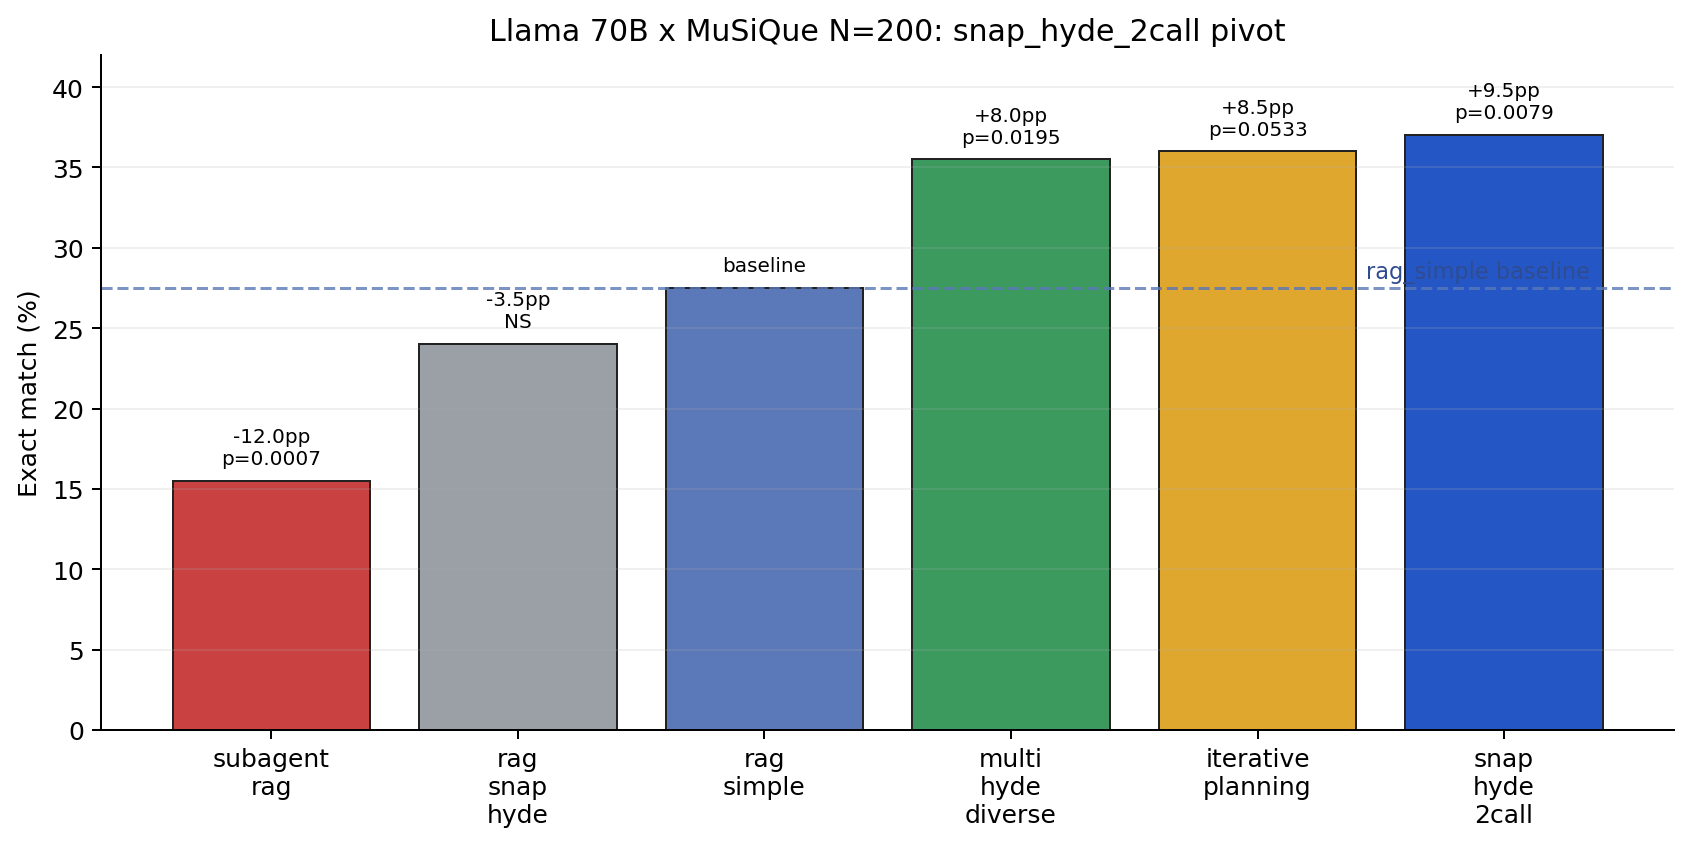
\includegraphics[width=0.82\textwidth]{08_musique_snap_hyde_2call_pivot.png}
  \caption{Current MuSiQue pivot for Llama 70B, $N=200$. The two-call
  snap-HyDE variant has the best point estimate and is significant versus
  \method{rag_simple}; it is not statistically separated from
  \method{multi_hyde_diverse} or \method{iterative_planning_table}.}
  \label{fig:musique_matrix}
\end{figure}

The retrieval-depth ablation shows why this is a retrieval-bottlenecked
regime. Restricting \method{rag_simple} from top-5 to top-1 passages drops EM
from 27.5\% to 13.0\% (-14.5pp, $p=4.18\times10^{-7}$). Across MuSiQue
methods, top-1 causes large drops of roughly 10--17pp. Passage count is
therefore a first-order variable; method choice matters, but only after the
system retrieves enough evidence.

\subsection{Cross-dataset bottleneck taxonomy}

\begin{table}[!htbp]
\centering
\caption{Retrieval-depth and method behavior across datasets.}
\label{tab:taxonomy}
\small
\begin{tabularx}{\textwidth}{>{\raggedright\arraybackslash}p{0.23\textwidth}
>{\raggedright\arraybackslash}p{0.36\textwidth}
>{\raggedright\arraybackslash}X}
\toprule
Dataset / model & Retrieval-depth diagnostic & Bottleneck read / caveat\\
\midrule
MuSiQue / Llama 70B (N=200) &
top-5 27.5\% to top-1 13.0\% (-14.5pp, $p=4.18{\times}10^{-7}$) &
Retrieval-depth limited; \method{snap_hyde_2call} adds a query-formulation
lift to 37.0\%.\\
BarExam / Gemma 4 26B (N=200 diagnostic) &
top-5 82.5\% to top-1 83.0\% (+0.5pp, $p=1.00$) &
Depth-flat; the full-corpus snap lift is modest and anchoring-driven, not
more-documents-driven.\\
CaseHOLD / Llama 70B (N=200) &
top-5 72.0\% to top-1 70.5\% (-1.5pp, $p=0.678$); two-call 69.5\% &
Answer-flat under current harness; do not cite gold-hit until repaired
CaseHOLD Chroma is rebuilt.\\
LegalBench-SCALR / Llama 70B (N=200) &
top-5 77.0\% to top-1 59.5\% (-17.5pp, $p=1.05{\times}10^{-8}$);
top-10 = 77.0\% &
Candidate-depth limited, then saturated by top-5 despite higher top-10
gold-hit.\\
HousingQA / Gemma 4 26B (N=200) &
top-1 50.5\% to top-10 58.0\% (+7.5pp, $p=0.0722$);
two-call 57.0\% &
Directional statutory retrieval-depth signal; state metadata and gold mapping
remain caveats.\\
\bottomrule
\end{tabularx}
\end{table}
\FloatBarrier

This table is the main conceptual result. Legal QA is not one regime. BarExam
and CaseHOLD are answer-flat under current depth and two-call probes, while
SCALR is retrieval-depth sensitive and HousingQA is a directional statutory
analogue. The CaseHOLD row is a negative control, not retrieval-recall
evidence: old logs report 0/200 gold-hit because the gold-option mapping was
not addressable until the repair. HousingQA is now a landed directional result
rather than merely a queued statutory test.

\section{Mechanism Analysis}

\subsection{Why the gold passage can be worse than snap-HyDE}

The BarExam golden-passage result initially looks paradoxical: if the system
is given the gold passage, why does it underperform \method{llm_only} and
\method{rag_snap_hyde}? The answer is that the gold passage is a control, not
an oracle. A single passage can be topically related without containing the
decisive rule, or it can emphasize a distractor doctrine that is plausible but
wrong for the fact pattern.

In the paired Gemma 4 26B BarExam audit, \method{llm_only} gets 79.75\% while
\method{golden_passage} gets 78.66\%. The transition table shows 96
\method{llm_only}-correct answers flipped wrong by the gold passage, compared
with 83 \method{llm_only}-wrong answers fixed by the passage. Meanwhile,
\method{rag_snap_hyde} reaches 81.17\%. A 30-case manual audit split the
paradox cases into topically irrelevant gold passages (30\%),
relevant-but-misapplied passages (50\%), and distractor or partial-rule
passages (20\%). Snap anchoring is therefore helpful but not magic:
\method{rag_snap_hyde} still follows the wrong gold-induced answer in 28 of
the 96 paradox cases. The mechanism is that snap-first reasoning gives the
model an initial legal answer to reconcile against evidence, rather than
letting one provided snippet dominate the first read.

\begin{figure}[!htbp]
  \centering
  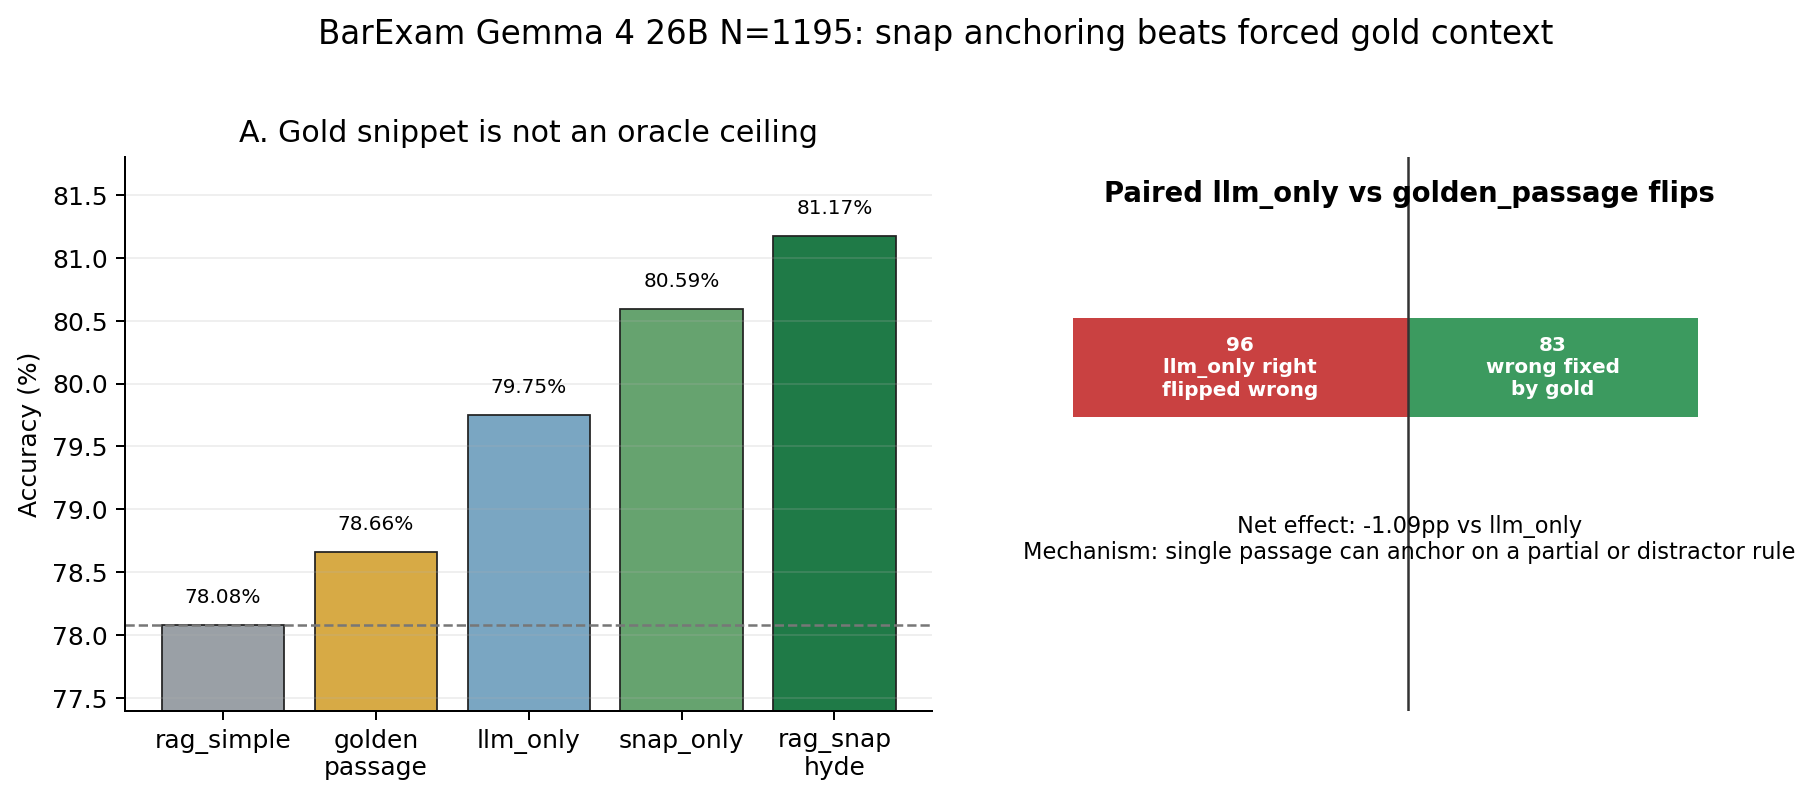
\includegraphics[width=0.86\textwidth]{11_barexam_golden_snap_mechanism.png}
  \caption{BarExam mechanism audit. The single gold-passage control is not an
  oracle ceiling: it flips more \method{llm_only}-correct answers wrong than
  wrong answers right, while snap-first methods recover some of that loss.}
  \label{fig:golden_mechanism}
\end{figure}
\FloatBarrier

\subsection{Gold context is task-dependent}

The same control reverses on MuSiQue. In a new Llama 70B N=200 paired
\method{golden_passage} run, providing the labeled gold passage reaches
56.5\% EM, compared with 27.5\% for \method{rag_simple} (+29.0pp,
$p=2.44\times10^{-13}$) and 37.0\% for \method{snap_hyde_2call} (+19.5pp for
gold over two-call, $p=8.07\times10^{-8}$). This does not make
\method{golden_passage} a deployable method; it is a control with access to
the answer-bearing context. But it shows why the BarExam result is not a
generic indictment of context injection. Gold context is useful when the model
lacks facts and harmful or noisy when a legal MC prior is already strong and
the provided snippet can anchor the wrong doctrine.

\subsection{Why snap-HyDE is model-conditional on MuSiQue}

The MuSiQue story is more retrieval-dominant. Llama 70B's snap-HyDE passages
improve gold-passage retrieval, and EM rises. Gemma 27B's snap-HyDE passages
move retrieval away from gold passages, and EM falls. This explains why
\method{snap_hyde_2call} is not a model-agnostic multi-hop cure: the method
helps only when the model can write a generated passage that matches the
corpus style and points retrieval toward the right evidence.

\begin{table}[!htbp]
  \centering
  \caption{MuSiQue snap-HyDE mechanism by model, $N=200$.}
  \label{tab:model_conditional}
  \small
  \begin{tabular}{lcccc}
  \toprule
  Model & RAG EM & 2-call EM & RAG gold-hit & 2-call gold-hit\\
  \midrule
  Llama 70B & 27.5\% & 37.0\% & 84.0\% & 86.5\%\\
  Gemma 27B & 28.5\% & 23.0\% & 84.0\% & 76.5\%\\
  \bottomrule
  \end{tabular}
\end{table}
\FloatBarrier

\subsection{Cost and practicality}

The final methods are intentionally much cheaper than the first agentic loop.
The full LangGraph agent used many calls per question and made debugging
difficult. \method{snap_hyde_2call} fixes the budget at two LLM calls per
question, with about 1,384 total tokens per question. It slightly exceeds
\method{multi_hyde_diverse} in EM at a similar two-call budget and far lower
latency, while \method{iterative_planning_table} spends 6.8 calls and roughly
2,929 tokens per question for a similar point estimate. Figure~\ref{fig:cost}
shows that the useful methods are not just the highest-accuracy methods; cost
per question matters.

\begin{figure}[!htbp]
  \centering
  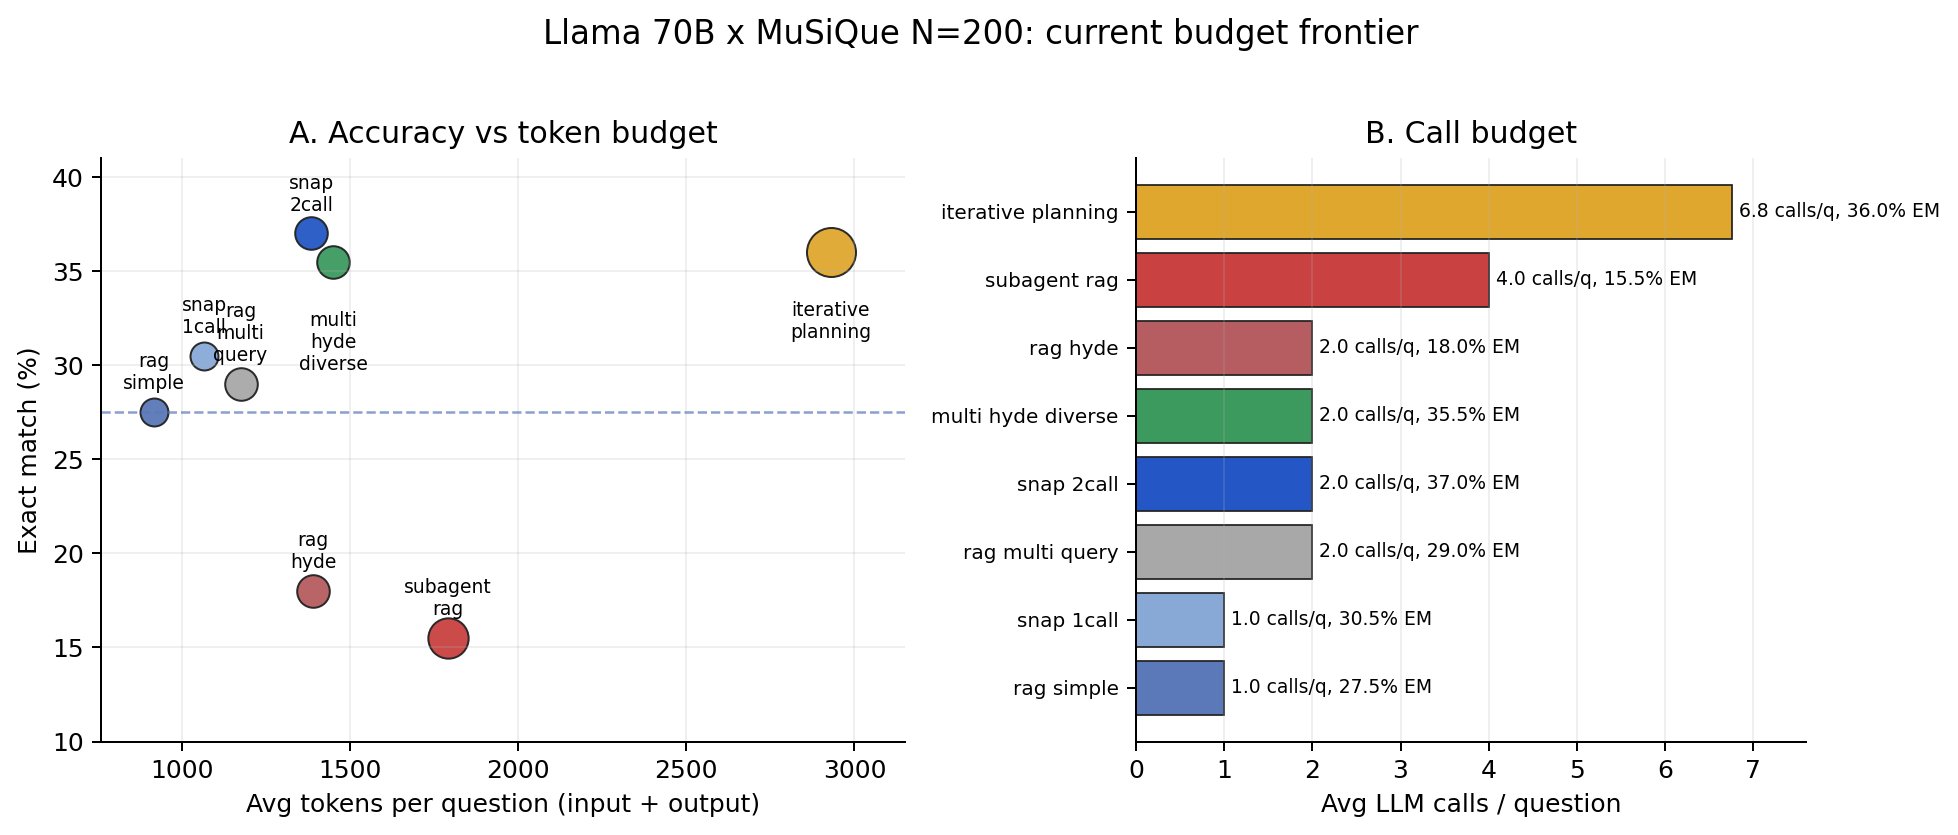
\includegraphics[width=0.90\textwidth]{10_musique_current_budget_frontier.png}
  \caption{Current cost vs.\ accuracy frontier on Llama 70B MuSiQue, $N=200$.
  Marker size tracks LLM calls. \method{snap_hyde_2call} is the best current
  point estimate at fixed two-call cost, while iterative planning spends far
  more calls for comparable EM.}
  \label{fig:cost}
\end{figure}
\FloatBarrier

\section{Limitations}

The strongest MuSiQue result is paired $N=200$, not a full-corpus run. It is
statistically significant, but a larger replicate would make the claim more
robust. The BarExam result is full-corpus and cross-size, but its effect size
is modest; it should be presented as a mechanism result rather than a dramatic
accuracy breakthrough. CaseHOLD previously lacked meaningful gold-option
retrieval instrumentation; we repaired the mapping, but new retrieval claims
require a rebuilt Chroma collection and fresh logs. HousingQA has landed only
as a directional N=200 diagnostic; the top-10 lift is suggestive, but state
metadata and weak gold-hit mapping still need a cleaner causal audit.

The method is also provider- and model-dependent. OpenRouter-served Gemma runs
showed runaway-loop behavior on iterative prompts, so Gemma results should
prefer cluster-served vLLM logs. More broadly, snap-HyDE depends on the model's
ability to generate a useful intermediate passage. If the generated passage is
off-style or wrong, retrieval can get worse.

\section{Conclusion}

The final project result is a more nuanced account of agentic legal RAG than
the original proposal. Heavy planning agents are not automatically better than
simple baselines. Retrieval is not automatically helpful, and gold context is
not an oracle. The useful direction is bottleneck-aware method selection:
multi-hop QA needs enough retrieved evidence and benefits from answer-shaped
retrieval; BarExam-style legal MC benefits more from snap-first reasoning and
careful reconciliation; holding-selection tasks need candidate-set diagnostics;
statutory QA likely needs metadata-aware retrieval. This is the strongest
story for a class report and the best foundation for future work on adaptive
legal RAG systems.

{\small
\bibliographystyle{plain}
\begin{thebibliography}{20}
\setlength{\itemsep}{0pt}
\setlength{\parskip}{0pt}

\bibitem{hyde2023}
Luyu Gao, Xueguang Ma, Jimmy Lin, and Jamie Callan.
Precise zero-shot dense retrieval without relevance labels.
\emph{ACL}, 2023.

\bibitem{query2doc2023}
Liang Wang, Nan Yang, and Furu Wei.
Query2Doc: Query expansion with large language models.
\emph{EMNLP}, 2023.

\bibitem{flare2023}
Zhengbao Jiang et al.
Active retrieval augmented generation.
\emph{EMNLP}, 2023.

\bibitem{iterretgen2023}
Zhihong Shao et al.
Enhancing retrieval-augmented large language models with iterative
retrieval-generation synergy.
\emph{EMNLP Findings}, 2023.

\bibitem{corag2025}
Zhiruo Wang et al.
CoRAG: A chain-of-retrieval augmented generation framework.
\emph{arXiv:2501.14342}, 2025.

\bibitem{specrag2025}
Zilong Wang et al.
Speculative RAG: Enhancing retrieval augmented generation through drafting.
\emph{ICLR}, 2025.

\bibitem{adaptiverag2024}
Soyeong Jeong et al.
Adaptive-RAG: Learning to adapt retrieval-augmented large language models
through question complexity.
\emph{NAACL}, 2024.

\bibitem{knowyourrag2025}
IBM Research.
Know Your RAG: Dataset and taxonomy for retrieval augmented generation.
\emph{COLING}, 2025.

\bibitem{grade2025}
GRADE.
Generating multi-hop QA with a reasoning-depth and semantic-distance
difficulty matrix.
\emph{EMNLP Findings}, 2025.

\bibitem{zheng2025legalretrievalbench}
Lucia Zheng, Neel Guha, and collaborators.
A reasoning-focused legal retrieval benchmark.
\emph{CS\&Law / arXiv:2505.03970}, 2025.

\bibitem{vaddi2026legal}
Vaddi.
Can small models reason about legal documents?
\emph{arXiv:2603.25944}, 2026.

\bibitem{musique2022}
Harsh Trivedi et al.
MuSiQue: Multihop questions via single-hop question composition.
\emph{TACL}, 2022.

\bibitem{legalbench2023}
Neel Guha et al.
LegalBench: A collaboratively built benchmark for measuring legal reasoning
in large language models.
\emph{arXiv:2308.11462}, 2023.

\end{thebibliography}
}

\end{document}
